\documentclass{article}
% load packages
\usepackage{amsmath}
\usepackage{amssymb}
\usepackage[hidelinks]{hyperref}
\usepackage{graphicx}
\usepackage[labelfont=bf]{caption}
% setup bibliography
\usepackage[sorting=none, style=numeric,backend=biber]{biblatex}
\addbibresource{aggregation.bib}

\renewcommand{\vec}[1]{\boldsymbol{#1}}

% ----------------------------- %
\title{Aggregating By Running Away!}
\author{Ole Schügl} 
% ----------------------------- %
\begin{document}
\maketitle

\section{Introduction}
Spatial pattern formation is a fascinating phenomenon that can be observed in a wide range of ecological settings, such as mussel beds, arid bushlands and bird flocks \autocite{liuPhaseSeparationDriven2016,rietkerkSelfOrganizationVegetationArid}.
Non-spatial modeling approaches can not capture the potential effects of spatial patterns on the system behaviour and it is therefore necessary to model space explicitly, when spatial structure is relevant for system functioning \cite{durrettImportanceBeingDiscrete1994}.
Besides being able to model the spatial arrangement of organisms in ecosystems, spatial modeling approaches have been able to show that pattern formation can have a positive impact on the stability of ecosystems \cite{durrettImportanceBeingDiscrete1994, vandekoppelExperimentalEvidenceSpatial2008,rietkerkEvasionTippingComplex2021,liuPatternFormationMultiple2014}. 
In mussel beds, for example, spatial patterns enable a combination of high growth and high survival which can not be achieved in homogeneous beds \autocite{vandekoppelExperimentalEvidenceSpatial2008}.

Although incorporating space is sometimes necessary, it introduces higher mathematical complexity and should not always be done.
To make this decision, it is important to understand when spatial structure impacts system functioning and to be explicit about the modeling assumptions and their justifications.
These considerations are explored in ref. \cite{durrettImportanceBeingDiscrete1994}, where four different approaches, two spatial models and two non-spatial models, for modeling the same system were analysed under three parameter choices and it was shown that no two models agree for all three parameter combinations.
Their results highlight how modeling results depend on the choice of the model and that it is important to select the right level of detail, depending on the modeling goals.

When trying to understand the spatial arrangement of ecological systems that exhibit pattern formation, it is clearly necessary to model space explicitly.
There are two main mechanisms that are usually put forward to explain the formation of patterns.
The first mechanism is based on the activation-inhibition principle described by Alan Turing \autocite{turingChemicalBasisMorphogenesis1952} and has been applied in a diverse range of ecosystems \autocite{rietkerkRegularPatternFormation2008}.
The activation-inhitition principle can be summarized as local excitation (e.g. reproduction) and global inhibition (e.g. long range competition for resources).

The second mechanism is based on the lesser known phase-separation priniciple developed by John Cahn and John Hilliard \autocite{cahnFreeEnergyNonuniform1958}. 
In ecological settings, this corresponds to density-dependent movement, where organisms switch between dispersive and aggregative movement as the density of neighbouring organisms of the same species increases \autocite{liuPhaseSeparationDriven2016}.
There is a diverse cast of organisms, among them certain species of mussels, slime moulds and bird- and fish flocks, whose spatial distribution can be explained by density-dependent movement \autocite{liuPhaseSeparationDriven2016}.

In this report, mathematical and numerical approaches for the modeling of spatial systems are explored by studying a simple model that leads to pattern formation based on a discrete version of the phase-separation principle.
Counter-intuitively, organisms form clusters only through diffusion and by moving faster when more organisms are around.
The model is simulated numerically, and the results are compared to density-independent diffusion and to the analytical results of a stability analysis of a PDE, describing an approximation of the discrete system with point densities.


\section{The Model}
First, a model for the density-dependent movement of organisms will be presented. 
The space in the model is a square with sidelength $1$ and periodic boundary conditions, which effectively means that organisms exist on a torus.

Since the focus is on movement, the number of organisms, $N$, is constant.
Initially, the organisms are distributed randomly in the environment. 
The position of all organisms is then updated at discrete time-steps by drawing a displacement from a normal distribution.
Mathematically, the change of the position $\vec{r}_i = (x_i, y_i)$ of individual $i$ can be described by
\begin{align}
    & x_i(t + dt) = x_i(t) + \sqrt{2D(N_R(\vec{r}_i, t)) dt} u_{i,x} \label{sysx}\\
    & y_i(t + dt) = y_i(t) + \sqrt{2D(N_R(\vec{r}_i, t)) dt} u_{i,y} \label{sysy}
\end{align}
where $u_{i,x}$ and $u_{i,y}$ are independent, normally distributed random numbers $\sim \mathcal{N}(0,1)$ and $D(N_R(\vec{r}_i, t))$ is a density-dependent diffusion rate.
The argument $N_R(\vec{r}_i, t)$ is the number of other organisms within a radius $R$ around the organism. 
For the diffusion rate function, we will use
\begin{equation}
    D(N_R(\vec{r}_i, t)) = D_0\left( \frac{N_R(\vec{r}_i, t)}{N\pi R^2} \right)^p.
\end{equation}
For a fixed interaction radius $R=0.1$, there are three parameters that influence the diffusion rate: $p, N$ and $D_0$.

In Fig. \ref{diffusion_rates}, the density-dependent diffusion rate as a function of the number of neighbours $\sqrt{2D(N_R) dt}$ is shown for a couple of different parameter values. 
This corresponds to the variance of the increments of the organism positions.
It can be seen, that the diffusion rate increases with the number of organisms in the neighbourhood.
Depending on the parameter $p$, this increase can be linear ($p=2$) or grow polynomially ($\mathcal{O}(n^{p/2})$). 
For larger values of $p$, the diffusion rate grows very fast, which will be important later.
The parameter $D_0$ shifts the curves up or down, and could be understood as a baseline diffusion rate.

In simulations, the impact of these parameters on pattern formation will be studied.

\begin{figure}[h]
    \centering
    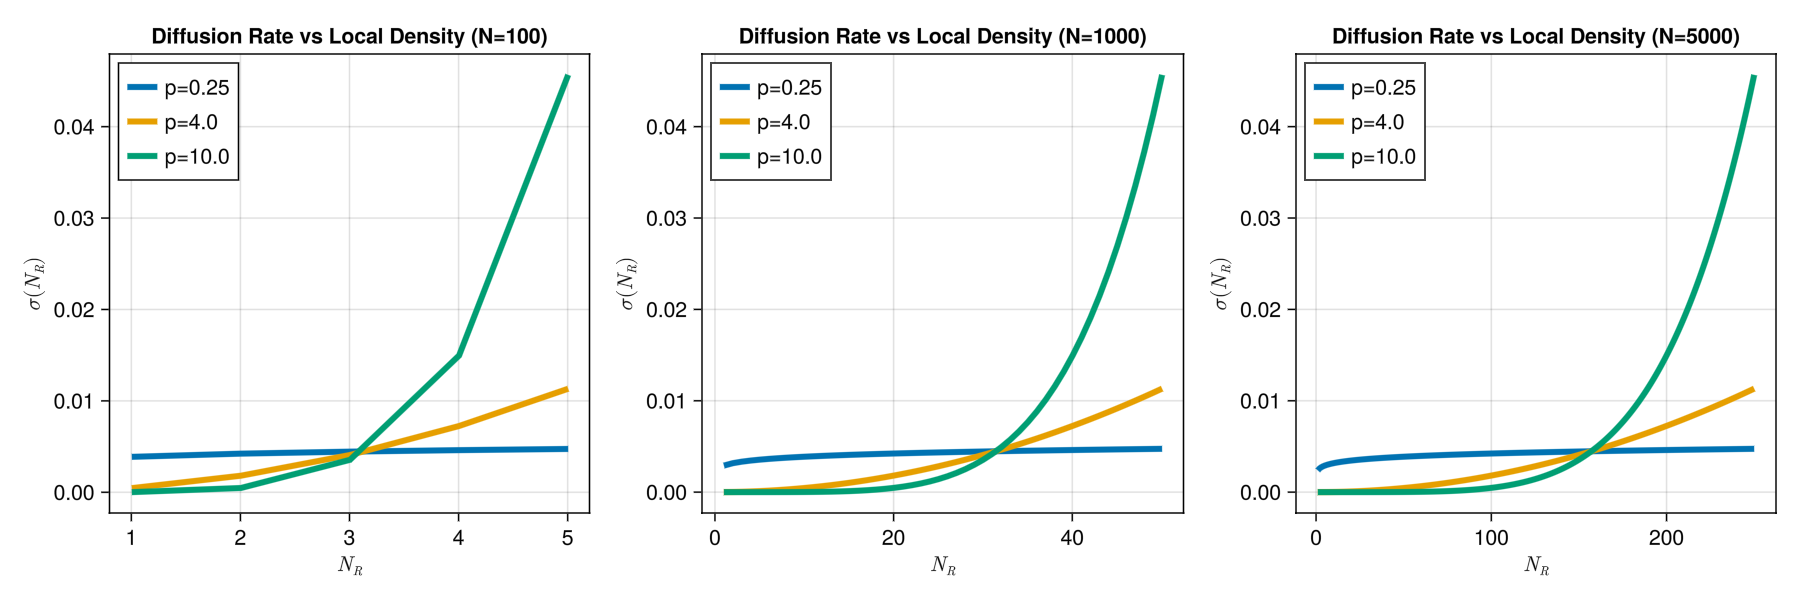
\includegraphics[width=1.0\linewidth]{img/diffusion_rates.png}
    \caption{Diffusion rate of an organism based on the number of other organisms within distance $R$ for $N=100$, $N=1000$, $N=5000$ and $p=0.25$, $p=4$, $p=10$ and $D_0 = 0.001$. Note that while the shape of the curves is the same, the number of organisms that can be within the radius to reach a certain diffusion rate increases with the total number of organisms.}
    \label{diffusion_rates} 
\end{figure}

\subsection{A Single Organism}
Before moving on to the simulations, the diffusion of independent organisms in space will be analysed.
As will be shown below, regular diffusion leads to organisms spreading out in space.
In general, diffusion is a process in which propability density evens out and it is therefore not obvious at all that clustering can be achieved through diffusive processes alone.

To see how organisms disperse under regular diffusion, consider a simple environment with only a single organism and a constant diffusion term. 
This can be recovered from the density-dependent diffusion rate by setting $p=0$.
For simplicity, it will be assumed that the environment is infinite, as opposed to the torus used in the simulations.\\
The walker position will change similiarly to before, but with a constant diffusion term
\begin{align}
    & x(t + dt) = x(t) + \sqrt{2D dt} u_x \label{single_x}\\
    & y(t + dt) = y(t) + \sqrt{2D dt} u_y
\end{align}
where $u_x, u_y$ are independent random numbers $\sim \mathcal{N}(0,1)$.\\
Let's consider the increments $dx(t+dt) = x(t + dt) - x(t)$.
Then 
\begin{equation*}
    x(t) = \sum_{\tau = 0}^{t/dt} dx(\tau) + x(0),
\end{equation*}
that is, the position of $x$ at time $t$ can be described by adding up the increments.
From Eq. \ref{single_x}, we can see that the increments are normally distributed with variance $2D dt$.
The distribution of the displacements $x(t) - x(0)$ is therefore a sum of normally distributed random variables, thus being again normally distributed with the variance being the sum of the variances 
\begin{equation*}
    x(t) - x(0) \sim \mathcal{N}(0,\sum 2D dt) =  \mathcal{N}(0,2Dt).
\end{equation*}
To make the following equations clearer, we will use $\tilde{x}(t) = x(t)-x(0)$ and $\tilde{y}(t) = y(t)-y(0)$ .
Using this, we calculate the mean squared displacement 
\begin{equation*}
    MSD(t) = \langle \tilde{x}^2(t) +\tilde{y}^2(t) \rangle = \langle \tilde{x}^2(t)\rangle + \langle\tilde{y}^2(t) \rangle.
\end{equation*}
Again we focus on the term involving $x$.
\begin{align*}
    \langle \tilde{x}^2(t)\rangle = \int_{-\infty}^{\infty} \tilde{x}^2 p(\tilde{x},t)d\tilde{x} = \int_{-\infty}^{\infty} \tilde{x}^2 \frac{1}{\sqrt{4\pi Dt}} e^{-\frac{\tilde{x}^2}{4Dt}}d\tilde{x}
\end{align*}
Solving this integral requires a few steps, that will be only briefly mentioned. 
First, we do a variable transformation by setting $u = \frac{\tilde{x}}{\sqrt{4Dt}}$. 
The integral then becomes
\begin{equation*}
    \frac{4Dt}{\sqrt{\pi}}\int_{-\infty}^{\infty} u^2  e^{-u^2}du.
\end{equation*}
This integral can be solved by partial integration and is equal to $\sqrt{\pi}/2$.
Thus, the final result is 
\begin{equation*}
    \langle \tilde{x}^2(t)\rangle = 2Dt.
\end{equation*}
For $\langle \tilde{y}^2(t)\rangle$, we get the exact same result, and the mean squared displacement is therefore
\begin{equation*}
    MSD(t) = \langle \tilde{x}^2(t)\rangle + \langle \tilde{y}^2(t)\rangle  = 4Dt.
\end{equation*}
These theoretical results are confirmed by simulations, where $1000$ independent organisms are initialized at the origin and the mean squared displacement is calculated over time.
The results can be seen in Figure \ref{regular_diffusion} and the MSD is in very good agreement with the theoretical prediction. 

\begin{figure}
    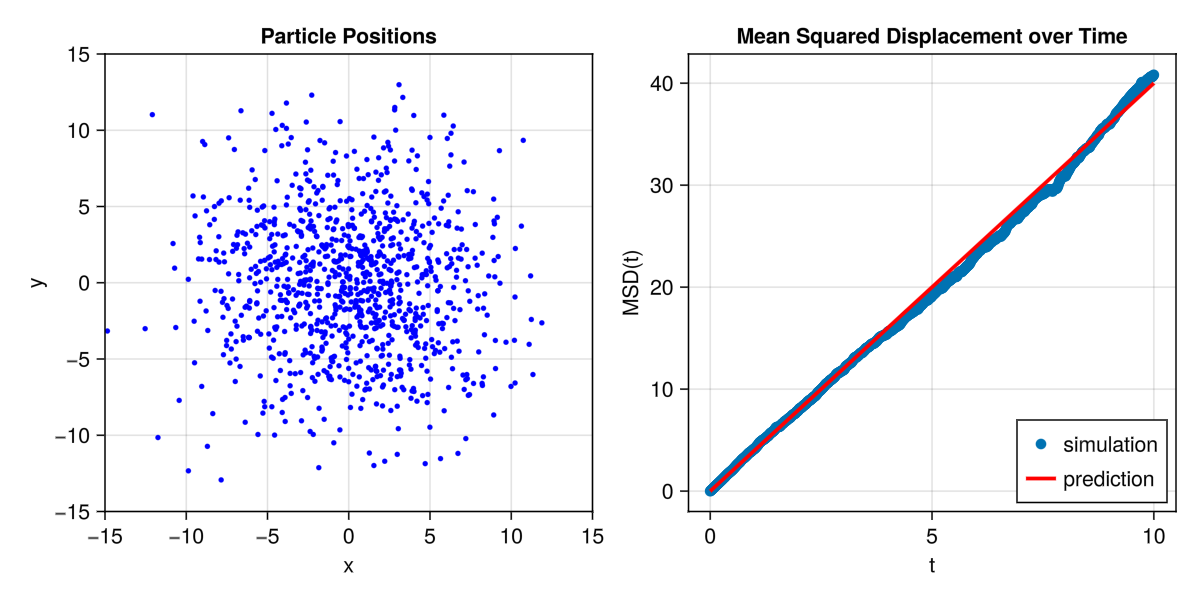
\includegraphics[width=1.0\linewidth]{img/diffusion36.png}
    \caption{MSD of organisms diffusing in space for a constant diffusion rate of $D=1$. The left panel shows the final distribution ($t=10$) of organisms and the right panel shows the MSD calculated at each point in time.}
    \label{regular_diffusion}
\end{figure}



\subsection{Stability Analysis}
Assuming that the population is large enough, we can approximate the dynamical system described by Eq. (\ref{sysx}), (\ref{sysy}) with a continuous density equation given by
\begin{equation} \label{pde}
    \frac{\partial\rho(\vec{r},t)}{\partial t} = \nabla^2[D(\rho_R)\rho(\vec{r},t)],
\end{equation}
where $\rho(\vec{r},t)$ now describes the point density at position $\vec{r}$ and time $t$ and
\begin{equation}
    D(\rho_R) = D_0 \left(\frac{\int_{R} \rho(\vec{r}',t)d\vec{r}'}{\pi R^2 \tilde{\rho}}\right)^p.
\end{equation}
The derivation of these equation from the discrete description are presented in ref. \autocite{lopezMacroscopicDescriptionParticle2006}.
The integral is taken over a disk of radius $R$ centered at $\vec{r}$. 
We will write the argument $\rho_R = \frac{\int_{R} \rho(\vec{r}',t)d\vec{r}'}{\pi R^2}$, which will make the subsequent analysis easier, because the function $D(\rho)=D_0 (\rho/\tilde{\rho})^p$ is simpler and does not contain non-local terms.

Following ref. \cite{lopezMacroscopicDescriptionParticle2006}, we do a linear stability analysis to understand under which conditions a uniform density is stable. 
This result will be used to find a suitable parameter range for simulations and is compared with the simulation results.

A small perturbation of the uniform density $\rho_0$ will be written as $\rho_0 + \epsilon \Psi$, giving
\begin{align}
    \frac{\partial[\rho_0 + \epsilon \Psi](\vec{r},t)}{\partial t} &= \nabla^2\left[D\left(\frac{\int_{R} [\rho_0+\epsilon \Psi](\vec{r}',t)d\vec{r}'}{\pi R^2}\right)[\rho_0+\epsilon \Psi](\vec{r},t)\right]\\
    &= \nabla^2\left[D\left(\rho_0+\frac{\epsilon\int_{R} \Psi(\vec{r}',t)d\vec{r}'}{\pi R^2}\right)[\rho_0+\epsilon \Psi](\vec{r},t)\right] \label{stability1}
\end{align}
Expanding $D$ in $\rho_0$ and setting $\Psi_R = \frac{\int_{R} \Psi(\vec{r}',t)d\vec{r}'}{\pi R^2}$, we get 
\begin{equation}
    D(\rho_0+\epsilon \Psi_R) = D(\rho_0) + \epsilon \Psi_R D'(\rho_0) + \mathcal{O}(\epsilon^2).
\end{equation}
Substituting this in Eq. (\ref{stability1}), gives
\begin{equation}
\nabla^2\left[\rho_0 D(\rho_0) + \rho_0\epsilon \Psi_R D'(\rho_0)+ D(\rho_0)\epsilon \Psi + \epsilon^2 \rho_0 \Psi_R D'(\rho_0) \Psi\right].
\end{equation}
The first term is $0$, since the density is uniform and we discard the last term because it is in $\mathcal{O}(\epsilon^2)$, leaving us with
\begin{equation} \label{pde_linear}
    \frac{\partial \Psi(\vec{r},t)}{\partial t} = \nabla^2\left[ D(\rho_0) \Psi(\vec{r},t)+\rho_0  D'(\rho_0)\Psi_R(\vec{r},t)  \right].
\end{equation}
Assuming a harmonic perturbation $\Psi(\vec{r}, t) = \Psi_0 e^{(\lambda t + i \vec{k} \cdot \vec{r})}$ and using Fourier analysis, we derive $\lambda$.
Depending on the sign of $\lambda$, the perturbations will either grow or decay over time.
We substitute $\Psi$ into Eq. \ref{pde_linear} to get
\begin{equation} \label{pde_substituted}
    \lambda \Psi(\vec{r},t) = D(\rho_0) \nabla^2\Psi_0 e^{(\lambda t + i \vec{k} \cdot \vec{r})} +  \rho_0  D'(\rho_0) \nabla^2\frac{\int_{R} e^{(\lambda t + i \vec{k} \cdot \vec{r'})}d\vec{r'}}{\pi R^2}.
\end{equation}
Writing $k=|\vec{k}|$, the first term on the RHS is $-k^2D(\rho_0)\Psi(\vec{r},t)$ while the second is more involved and calculated below.
We have 
\begin{equation} 
 \nabla^2\frac{\int_{R} e^{(\lambda t + i \vec{k} \cdot \vec{r'})}d\vec{r'}}{\pi R^2} = \nabla^2e^{(\lambda t + i \vec{k} \cdot \vec{r})}\frac{\int_{\mathbb{R}^2}\chi_{|\vec{r}-\vec{r'}|<R} \cdot e^{ i \vec{k} \cdot (\vec{r'}-\vec{r})}d\vec{r'}}{\pi R^2}.
\end{equation}
The integral is now independent of space and is the Fourier transform of the 2D top hat function, i.e.
\begin{equation} 
    \nabla^2e^{(\lambda t + i \vec{k} \cdot \vec{r})}\frac{\int_{\mathbb{R}^2}\chi_{|\vec{r}-\vec{r'}|<R} \cdot e^{ i \vec{k} \cdot (\vec{r'}-\vec{r})}d\vec{r'}}{\pi R^2} = -k^2\Psi(\vec{r},t) \hat{G}(\vec{k}).
   \end{equation}
In ref. \cite{lopezMacroscopicDescriptionParticle2006}, they state that $\hat{G}(\vec{k}) = 2J_1(kR) / kR$, which we use to find a value of $\lambda$,
\begin{equation}
    \lambda(\vec{k}) = -D_0 k^2\left(1 + \frac{2pJ_1(kR)}{kR}\right),
\end{equation}
where $J_1$ is the first-order Bessel function.
The paper also states a critical value of $p\sim 7.6$, for which $\lambda $ becomes positive, though there is no discussion about the value of $k$ for which this is attained. 
This means that the onset of pattern formation for the PDE occurs around $p_c \sim 7.6$ and independent of $D_0$, because the uniform distribution loses its stability.


\subsection{Pairwise Correlation Function}
The pairwise correlation function (PCF) and the closely related Ripley's K function are popular tools for quantifying the characteristics of point patterns \autocite{wiegandRingsCirclesNullmodels2004}. 
They are based on the pairwise distances between all points and provide information about the spatial scales of the patterns as well.
The PCF, denoted by $g(d)$, measures the average number of points at a distance $d$ from a randomly selected point.
Because there is a finite number of points, we look at rings of finite width and calculate the PCF based on the number of points within a small ring.
The PCF is normalized such that a completely random distribution of points corresponds to $g(d) \equiv 1$.

To calculate $g(d)$, the pairwise distances between all points is calculated and results are binned into a histogram, in our case with $200$ evenly spaced bins, which corresponds to the rings mentioned above.
The normalization is then 
\begin{equation}
    g(d) = \frac{W(d)}{2\pi d  N^2 \delta d},
\end{equation}
where $W(d)$ is the average number of points at a distance between $d$ and $d + \delta d$ from a randomly chosen point \cite{52PairCorrelation}.
Because the simulation is on a torus, no edge effects occur for $d < 0.5$.

The PCF will be calculated for the final distribution of points in the simulations (see below), and used as an indicator to classify the observed pattern.
While I have not found any source for this and the statistical significance of this approach is not clear, the MSD between the PCF and $f(d) \equiv 1$ seems to be a good measure of how different a pattern is from a completely random distribution and will be denoted by $MSD(g)$. 
Since no clear regular patterns were noted in the simulations, a high value of $MSD(g)$ will be interpreted as an indication of cluster formation, while a low value of $MSD(g)$ will be interpreted as an indication of random distribution.

\subsection{Simulations}
\begin{figure}
    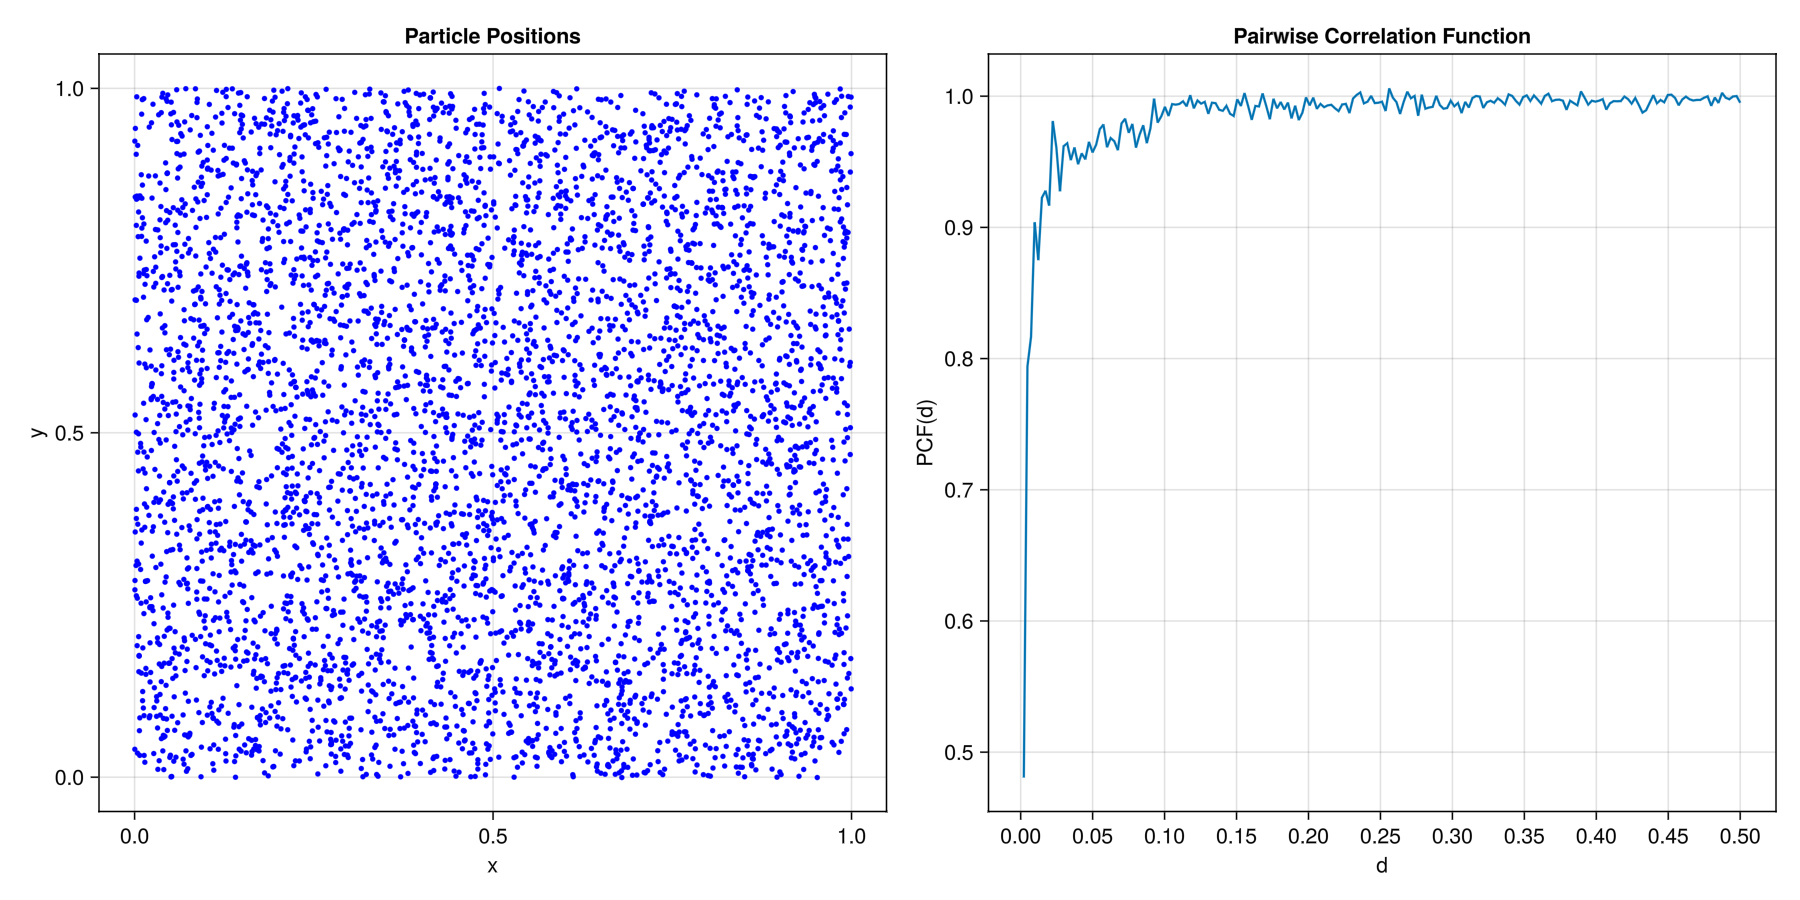
\includegraphics[width=0.8\linewidth]{img/rp156_N5000_D01_p4.png}
    \caption{Results of the simulation with $N=5000$, $p=4$, $D_0=0.01$. The left panel shows the final distribution of the organisms and the right panel shows the PCF of this configuration. The organisms are randomly distributed and the PCF is close to $1$ for all distances.}
    \label{random}
\end{figure}
Numerical simulations of the system with density-dependent diffusion rates were implemented in the programming language julia.
To keep things managable, three population sizes were simulated, $N_1=200, N_2 = 1000, N_3 = 5000$.
For each population size, the simulation was run for a number of values of the parameters $p$ and $D_0$.
Based on the stability analysis, for population sizes $N_1$ and $N_2$, $40$ evenly spaced values between $5$ and $10$ were simulated for the parameter $p$ and $10$ values were used for the largest population size $N_3$.
The parameter $D_0$ was simulated across a broader range, from $10^{-1}$ to $10^{-4}$ and for population sizes $N_1$ and $N_2$, $40$ logarithmically evenly spaced values were used, while for population size $N_3$, $10$ values were used again.
A smaller number of parameters was simulated for population size $N_3$, because of the much higher computation time.
The initial positions of the organisms was drawn from a uniform distribution on a square of sidelength 1.

To allow patterns to form, the simulation was run for $n=2000$ steps. 
At the end of the simulation, the PCF is calculated and $MSD(g)$ is recorded as a measure to indicate pattern formation and plotted as a heatmap for all parameter values (See Figure \ref{heatmap1000}).

Because it is very insightful to watch the simulation play out live, the code provided alongside the report has the option to see the simulation play out in real-time.

\section{Simulation Results} \label{secres}

Depending on the simulation parameters, the system ends up in one of two possible configurations: clumped or randomly distributed.

% first describe random pattern.
A random configuration is shown in Figure \ref{random}, alongside the PCF for the largest population size $N_3=5000$. 
No clear pattern is visible and the PCF is close to the line $y=1$.
For distances below the interaction range $R=0.1$, the PCF lies a little bit below $1$, which could indicate a slightly overdispersed pattern, though I am not sure if this is significant.

% clumped pattern
In Figure \ref{clumped}, a clumped configuration of organisms and the PCF can be seen, as before.
The clumps are very evenly spaced, forming a grid-like pattern. 
The PCF has clearly distinguished peaks and valleys, from which characteristic lengths in the system can be determined.
The first time the PCF drops below $1$ is for a distance slightly below $0.05$ and the PCF rises above $1$ for distances slightly above $0.1$, which is also the interaction range, $R$, of the organisms.
While for $N_2=1000$ a similar structure can be seen just with fewer individuals per clump, for $N_1=200$ cluster sizes are so small (at most $3$ organisms), that no real patterns can be observed and the PCF is very noisy.
% resultplot 51 - 74 
\begin{figure}
    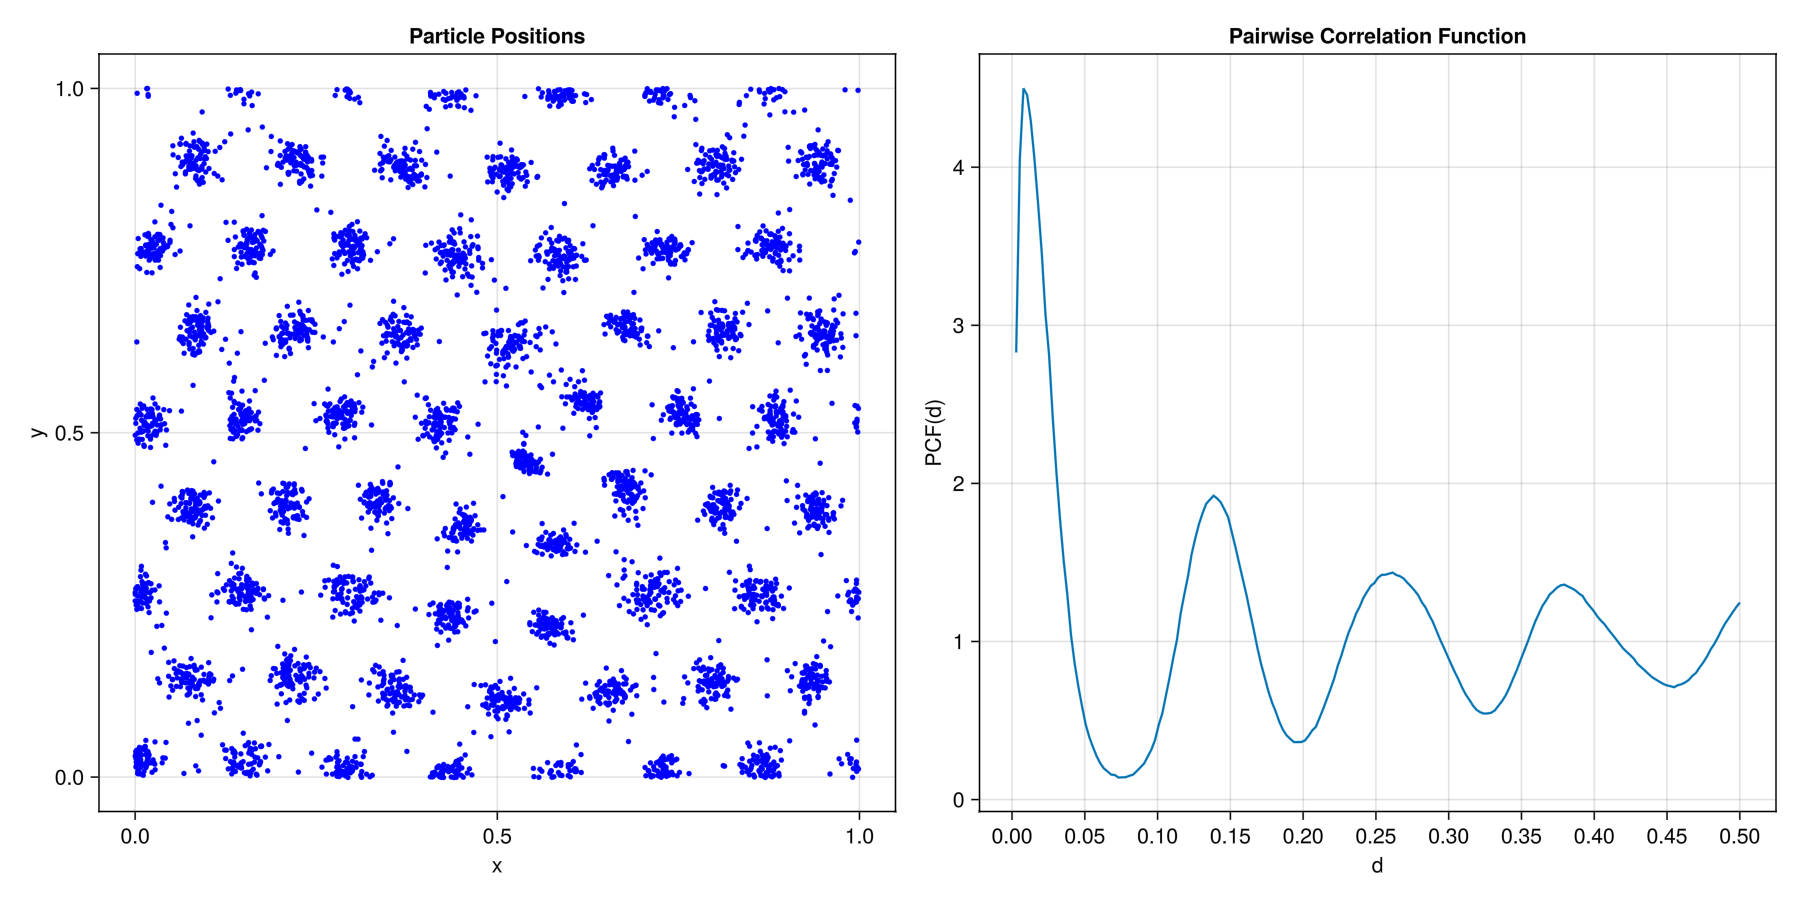
\includegraphics[width=0.8\linewidth]{img/rp159_N5000_D01_p8.png}
    \caption{Results of the simulation with $N=5000$, $p=8$, $D_0=0.01$. The left panel shows the final distribution of the organisms and the right panel shows the PCF of this configuration. Clusters have formed and the PCF deviates strongly from $1$.}
    \label{clumped}
\end{figure}

To find the range of parameters where clumped patterns occur, the indicator $MSD(g)$ is calculated for a large number of parameters and plotted as a heatmap in Figure \ref{heatmap1000}. 
A slightly noisy transition occurs around $p=7$ from small values of $MSD(g)$ to large values of $MSD(g)$, but in contrast to what the stability analysis of the density-based approximation of this system predicts, there is clearly a dependence on the parameter $D_0$ as well. 
For large value of $D_0$, no clumped patterns occur anymore.
Additionally, very small values of $D_0$ also seem to lead to random patterns, however, this is an artifact of not running the simulation for long enough. 
In this scenario, the organisms move very slowly and take much longer to settle into clumped patterns.
For $N=5000$, the $10\times10$ grid of parameter choices seems to behave similarly, although the resolution is not high enough to say this for sure.
For $N=200$, the heatmap is extremly noisy, making it difficult to point to a clear transition.

There is a transition region where neither a random nor a clumped distribution is stable, for example for $N=1000, p=6.5, D_0=0.001$.
\begin{figure}
    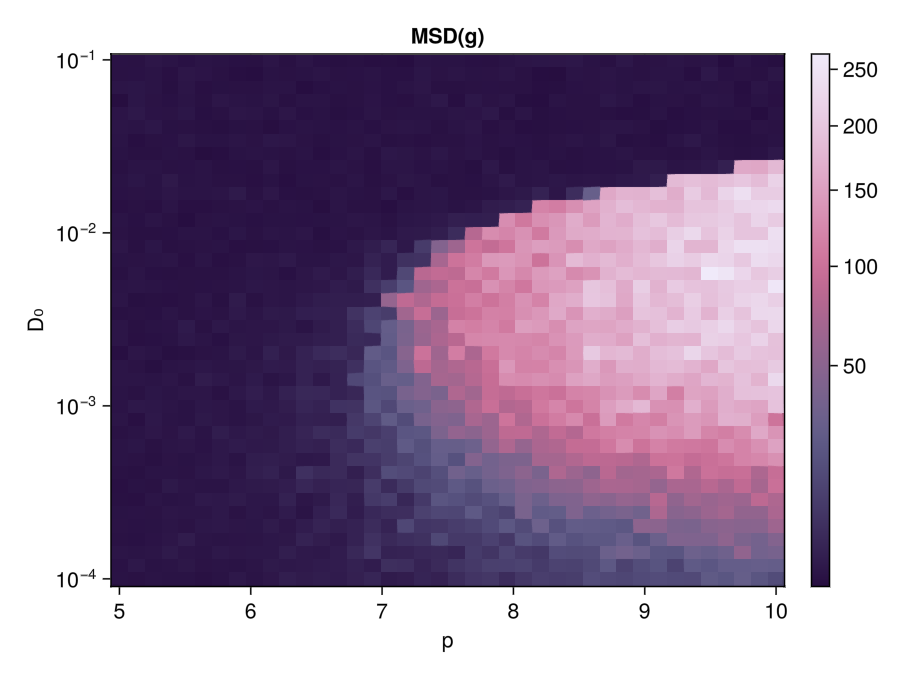
\includegraphics[width=0.8\linewidth]{img/hm1.png}
    \caption{Value of $MSD(g)$ for a grid of parameter choices and $N=1000$. Brighter values indicate clustering while dark purple indicates random distributions. } 
    \label{heatmap1000}
\end{figure}

\section{Discussion}
We have seen a counter-intuitive mechanism that leads to pattern formation by organisms that move faster when more other organisms are around.
Additionally, we have seen some theoretical and numerical approaches for analysing the distribution of spatial patterns. 

A speculative explanation of what is required for pattern formation is provided, building upon the observation of real-time simulations and the previous analysis.
It boils down to a combination of a low baseline diffusion rate and a strong increase in the diffusion rate with a growing number of organisms within the interaction range.

A low baseline diffusion rate ensures that the clumps don't just diffuse away because the organisms move only slowly within clusters.
As we have seen in an earlier section, the mean displacement of an organism due to a constant diffusion rate grows like $\sqrt{4Dt}$. 
Thus an organism inside a cluster with an approximatly constant number of organisms would leave the cluster after some amount of time, but this could take a long time provided $D$ is small enough.

The second aspect allowing pattern formation is a rapid increase in the diffusion rate with an increasing number of organisms within the interaction range. 
As we have noted, clumps are slightly further apart than the interaction range, meaning that organisms within a cluster only interact within that cluster.
However, an organism that leaves the cluster through diffusion suddenly is within the interaction range of multiple clusters and has more organisms within their interaction range. 
Because the diffusion rate grows rapidly with an increase in neighbours, the organism moves very fast until it jumps into a cluster again where the diffusion rate becomes much lower again.
Since organisms take much longer to diffuse out of a cluster, than it takes them to be captured again, the clusters are stable.

While this does not entirely explains the initial formation of patterns, it explains why patterns are stable once they emerge.

The continuous approximation (Eq. \ref{pde}), predicts that the uniform solution loses stability for $p=7.6$ and independent of $D_0$. 
The discrete dynamics, on the other hand, shows a dependence on $D_0$ and an earlier transition, with the random distribution becoming unstable as early as $p=6.5$.
While the continuous approximation can provide some insights into the behavior of the discrete model, there are qualitative differences in the resulting dynamics, again highlighting the findings of ref. \autocite{durrettImportanceBeingDiscrete1994}.

While this simple model is unlikely to be a realistic description of any real ecosystem, the continuous description used in the stability analysis, and which is derived from the model studied in this report, has been modified and applied in ecological 
settings to mussel beds and bacteria, among others \autocite{liuPhaseSeparationDriven2016,liuPhaseSeparationExplains2013}.
Additionally, the methods presented here, like the stability analysis and the PCF, can be used to study many spatial systems.

% Additionally, the stability analysis indicates for which parameter values the initial uniform distribution becomes unstable, which allows clusters to form in the first place. 
% The onset of pattern formation already occurs for slightly smaller values of $p$ than the predicted value of $p_c =7.6$ where a transition region exists. 
% In this region, for example for $p=7.4$ and $D=0.01$, clusters start to form but dissolve again quickly and no stable pattern emerges.

% While not being the focus of this report, a short discussion about the number of clusters and their distances is presented.
% Without exactly measuring the size of clusters, they seem to have a diameter of around $0.04-0.05$ and the distance between clusters is around $0.12$, which indicates that clusters are spaced such that the organisms on the outer parts of a cluster already are within range of organisms of the next cluster. 
% The clusters seem to be arranged along prallel lines and there are three directions of lines. 
% Approximately $60-90$ clusters should be possible, meaning that for $1000$ organisms, the average cluster size is around $10-20$ organisms.
% Importantly, the number of clusters and their distances does not seem to depend on the number of organisms.
% Parameter choices that lead to clustering should have low diffusion rates while an organism is within the interaction range of a number of organisms that is around the average cluster size and then increase rapidly as the number of organisms within the interaction range grows to 2 times the average cluster size. 

% This raises the question whether the same interaction range can lead to differently spaced and sized clusters or whether the interaction range forces a certain length scale on the system, and therefore also a certain average cluster population.

\printbibliography
\end{document}